\section{弾性による影響}

粘性による影響では説明が十分にできない
球の落下によって生じる応力$\tau_\text{U}$に関して,式(\ref{eq:tauU})
といった式で近似できる.

\ref{sec:elasticity}節にて,粘性と弾性の優位が入れ替わる応力$\tau_\text{0}$を求めた.この応力$\tau_\text{0}$より大きいと,粘性の影響が大きい.一方で,小さい場合は弾性に寄る影響が大きい.この応力$\tau_\text{0}$と球の落下による応力$\tau_\text{U}$の比である,$\tau_\text{U}/\tau_\text{0}$を用いて,超音波照射による球の高速化度合いを整理する.この比が1より大きいと粘性による影響が,1より小さいと弾性による影響が大きい.この整理を行うことで,弾性による超音波照射された落下球の高速化度合いへの影響を考えることができる.応力比と高速化度合いの関係性を示した結果をFig.\ref{fig:elastcity}に示す.

\begin{figure}[h]
    \centering
    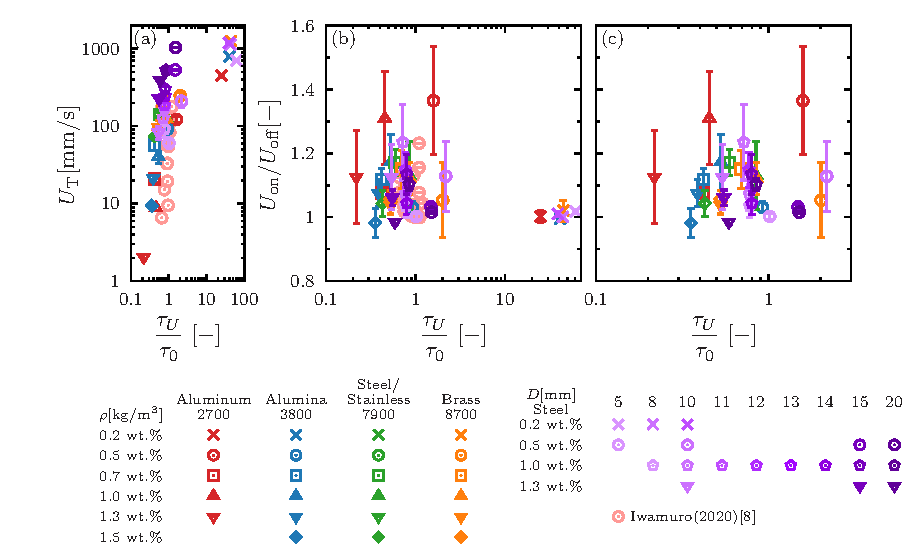
\includegraphics[width=1.0\textwidth]{5-Results/elastcity.eps}
    \caption{Relationship between velocity ratio and elasticity ratio $\tau_\text{U}/\tau_\text{0}$.}
    \label{fig:elastcity}
\end{figure}

\begin{figure}[h]
    \centering
    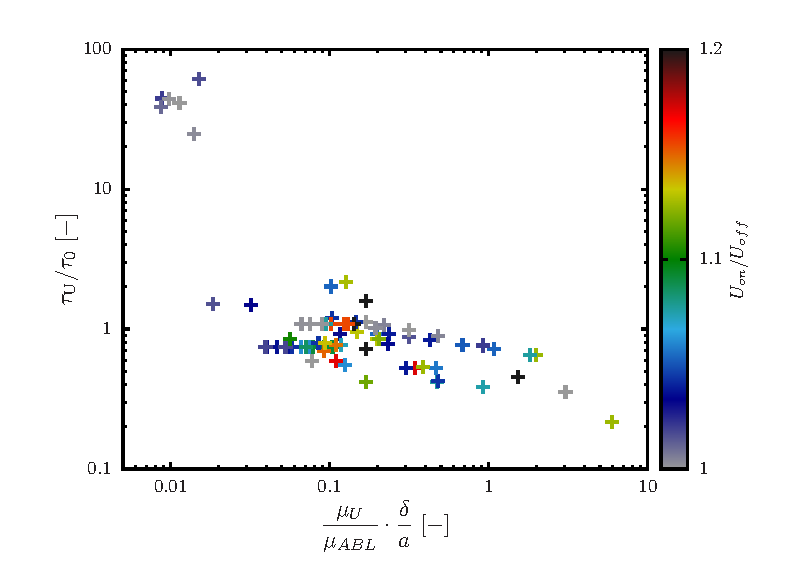
\includegraphics[width=1.0\textwidth]{5-Results/elastcity_color.eps}
    \caption{}
    \label{fig:elastcityColor}
\end{figure}
